\documentclass{mwart} 
\usepackage[polish]{babel} 
\usepackage[utf8]{inputenc} 
\usepackage{polski} 
\usepackage[T1]{fontenc} 
\usepackage{graphicx}

\usepackage[margin=1cm]{geometry}




\frenchspacing 

\usepackage{indentfirst} 
\title{\Huge{Sprawozdanie z laboratorium nr 9\\
Przeszukiwania grafów }}
\author{Agnieszka Wiśniewska, nr albumu: 200466}

\begin{document}

\maketitle

\section{Wprowadzenie}
Graf jest strukturą danych do reprezentacji obiektów, między którymi występują różne zależności. Podstawowymi elementami grafu są wierzchołki połączone ze sobą krawędziami. Graf nieskierowany (obecny program) to taki, w którym krawędzie można przebywać w obie strony (kolejność wierzchołków w parze definiującej krawędź nie jest istotna). Wagi są to wartości związane z krawędziami.\\
W tym sprawozdaniu omówione zostaną trzy sposoby wyszukiwania ścieżek - za pomocą przeszukiwania w głąb, wszerz oraz za pomocą algorytmu A*.

\section{Przeszukiwania grafów}
Zaimplementowano trzy algorytmy przeszukiwania grafów:\\
\subsection{DFS - przeszukiwanie w głąb}
Z przeszukiwaniem w głąb mamy do czynienia, gdy do implementacji zbioru wierzchołków do odwiedzenia używamy stosu. Określenie "przeszukiwanie w głąb" bierze się stąd, że zawsze próbujemy kontynuować przeszukiwanie z najpóźniej odkrytego wierzchołka, czyli z tego, który znajduje się na szczycie stosu. Przeszukiwanie w głąb najprościej jest opisać rekurencyjnie. 

\subsection{BFS - przeszukiwanie wszerz}
Przeszukiwanie wszerz różni się od przeszukiwania w głąb użytą strukturą danych. W przypadku przeszukiwania wszerz możemy skorzystać np.: z kolejki (tak jak zostało zaimplementowane w programie). Przeszukiwane są wszystkie wierzchołki grafu sąsiadujące z wierzchołkiem początkowym, następnie sprawdzane są kolejne, aż do natrafienia na ostatni wierzchołek. Należy uważać, by nie wracać do wierzchołków wcześniej odwiedzonych (każdy można odwiedzić tylko raz). Jeżeli po przeszukaniu wszystkich wierzchołków nie znajdziemy stanu końcowego oznacza to, że nie istnieje droga między szukanymi wierzchołkami.

\subsection{A*}
A* służy do wyszukiwania najkrótszej ścieżki w grafie ważonym pomiędzy punktem startowym, a docelowym. Algorytm tworzy ścieżkę, za każdym razem wybierając wierzchołek x z dostępnych w danym kroku niezbadanych wierzchołków tak, by wartość funkcji f(x)=g(x)\footnote{g(x) to droga pomiędzy wierzchołkiem początkowym a wierzchołkiem x} +h(x)\footnote{h(x) to przewidywana przez heurystykę droga od x do wierzchołka docelowego} była jak najmniejsza. W każdym kroku algorytm dołącza do ścieżki wierzchołek o najniższym współczynniku f. Kończy w momencie natrafienia na wierzchołek będący wierzchołkiem docelowym.

\newpage
\section{Porównanie czasu działania algorytmów}

\begin{figure}[!htp]
\centering
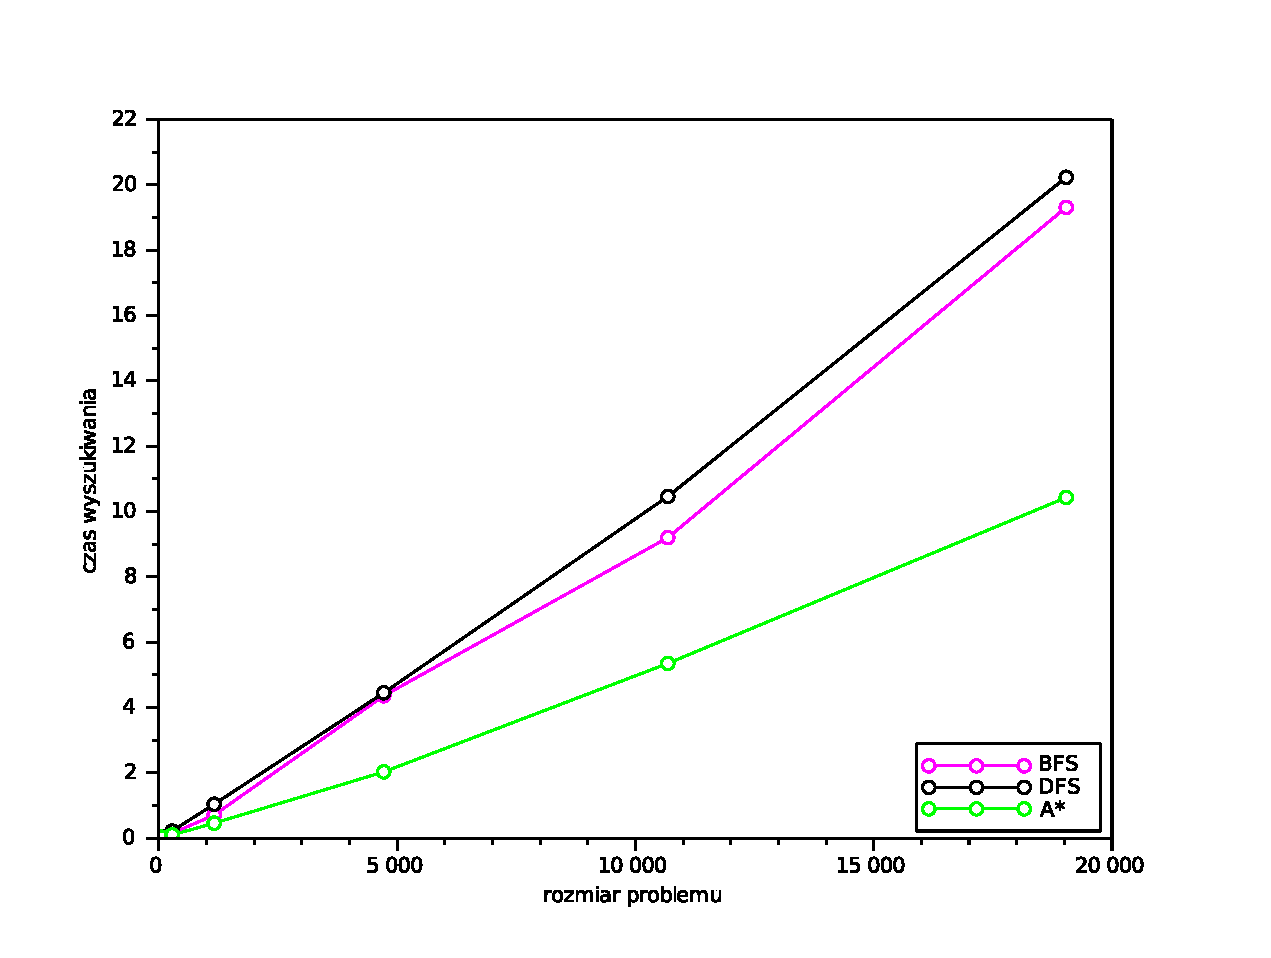
\includegraphics[width=0.95\textwidth]{alg.pdf}
\caption{Zależność czasu wykonywania algorytmów od rozmiaru problemu dla zaimplementowanych przeszukiwań. \label{alg}} 
\end{figure}


Jak widać na rysunku \ref{alg} najszybciej ścieżkę pomiędzy wierzchołkiem docelowym odnajduje A*.

\section{Podsumowanie i wnioski}
\begin{itemize}
\item Udało się osiągnąć rezultat zgodny z oczekiwaniami - najlepszym rozwiązaniem okazał się A*. Jest to algorytm, który nie sprawdza wszystkich wierzchołków, jednak szacuje drogę do pokonania - jak widać na powyższym rysunku jest on zdecydowanie szybszy od algorytmów przeszukiwania w głąb i wszerz.
\item Algorytm A* jest kompletny i w każdym przypadku znajdzie optymalną drogę i zakończy działanie - o ile taka droga istnieje. 
\item Algorytm A* jest optymalny dla danej heurystyki, co znaczy, że nie istnieje inny algorytm, który z pomocą tej samej heurystyki odwiedziłby mniej wierzchołków niż A*.
\item Algorytmy DFS oraz BFS mogą działać równie szybko, jednak tylko w przypadku odpowiedniego doboru grafu.


\end{itemize}




\end{document}